\documentclass[12pt,]{book}
\usepackage{lmodern}
\usepackage{setspace}
\setstretch{1}
\usepackage{amssymb,amsmath}
\usepackage{ifxetex,ifluatex}
\usepackage{fixltx2e} % provides \textsubscript
\ifnum 0\ifxetex 1\fi\ifluatex 1\fi=0 % if pdftex
  \usepackage[T1]{fontenc}
  \usepackage[utf8]{inputenc}
\else % if luatex or xelatex
  \ifxetex
    \usepackage{mathspec}
  \else
    \usepackage{fontspec}
  \fi
  \defaultfontfeatures{Ligatures=TeX,Scale=MatchLowercase}
    \setmainfont[]{Montserrat}
\fi
% use upquote if available, for straight quotes in verbatim environments
\IfFileExists{upquote.sty}{\usepackage{upquote}}{}
% use microtype if available
\IfFileExists{microtype.sty}{%
\usepackage{microtype}
\UseMicrotypeSet[protrusion]{basicmath} % disable protrusion for tt fonts
}{}
\usepackage[marginpar=2cm, top=3cm, bottom=4cm]{geometry}
\usepackage{hyperref}
\hypersetup{unicode=true,
            pdfborder={0 0 0},
            breaklinks=true}
\urlstyle{same}  % don't use monospace font for urls
\usepackage{natbib}
\bibliographystyle{plain}
\usepackage{longtable,booktabs}
\usepackage{graphicx,grffile}
\makeatletter
\def\maxwidth{\ifdim\Gin@nat@width>\linewidth\linewidth\else\Gin@nat@width\fi}
\def\maxheight{\ifdim\Gin@nat@height>\textheight\textheight\else\Gin@nat@height\fi}
\makeatother
% Scale images if necessary, so that they will not overflow the page
% margins by default, and it is still possible to overwrite the defaults
% using explicit options in \includegraphics[width, height, ...]{}
\setkeys{Gin}{width=\maxwidth,height=\maxheight,keepaspectratio}
\IfFileExists{parskip.sty}{%
\usepackage{parskip}
}{% else
\setlength{\parindent}{0pt}
\setlength{\parskip}{6pt plus 2pt minus 1pt}
}
\setlength{\emergencystretch}{3em}  % prevent overfull lines
\providecommand{\tightlist}{%
  \setlength{\itemsep}{0pt}\setlength{\parskip}{0pt}}
\setcounter{secnumdepth}{5}
% Redefines (sub)paragraphs to behave more like sections
\ifx\paragraph\undefined\else
\let\oldparagraph\paragraph
\renewcommand{\paragraph}[1]{\oldparagraph{#1}\mbox{}}
\fi
\ifx\subparagraph\undefined\else
\let\oldsubparagraph\subparagraph
\renewcommand{\subparagraph}[1]{\oldsubparagraph{#1}\mbox{}}
\fi

%%% Use protect on footnotes to avoid problems with footnotes in titles
\let\rmarkdownfootnote\footnote%
\def\footnote{\protect\rmarkdownfootnote}

%%% Change title format to be more compact
\usepackage{titling}

% Create subtitle command for use in maketitle
\newcommand{\subtitle}[1]{
  \posttitle{
    \begin{center}\large#1\end{center}
    }
}

\setlength{\droptitle}{-2em}
  \title{}
  \pretitle{\vspace{\droptitle}}
  \posttitle{}
  \author{}
  \preauthor{}\postauthor{}
  \date{}
  \predate{}\postdate{}

% Améliore l'esthétique de la police
\usepackage{lmodern}

%Packages pour créer des tableaux 
\usepackage{longtable} % Pour des tableaux dont la longueur dépasse une feuille A4
\usepackage{tabularx} % Pour des tableaux à largeur définie
\usepackage{array} % Pour améliorer la qualité typographique des tableaux.
\usepackage{siunitx}
\usepackage{pdfpages}

\usepackage{amsthm}
\newtheorem{theorem}{Theorem}[chapter]
\newtheorem{lemma}{Lemma}[chapter]
\theoremstyle{definition}
\newtheorem{definition}{Definition}[chapter]
\newtheorem{corollary}{Corollary}[chapter]
\newtheorem{proposition}{Proposition}[chapter]
\theoremstyle{definition}
\newtheorem{example}{Example}[chapter]
\theoremstyle{definition}
\newtheorem{exercise}{Exercise}[chapter]
\theoremstyle{remark}
\newtheorem*{remark}{Remark}
\newtheorem*{solution}{Solution}
\begin{document}

%Page de garde
\begin{titlepage}
\frontmatter
\begin{figure}[t]

\includegraphics[width=5cm]{figures-ext/LogoParisDescartes}
\end{figure}
\begin{center}
UNIVERSITÉ PARIS DESCARTES \\
\vspace*{1cm}
\textbf{ED 474 Frontières du vivant}\\
\vspace*{0,5cm}
\textit{Institut Curie, PSL Research University, Mines Paris Tech, Inserm U900 \\Paris, France}\\
\vspace*{1cm}
\LARGE{\textbf{COMPUTATIONAL DECONVOLUTION OF CELL AND ENVIRONMENT SPECIFIC SIGNALS AND
THEIR INTERACTIONS FROM COMPLEX MIXTURES IN BIOLOGICAL SAMPLES}}\\
\large{\textbf{Par Urszula Czerwińska}}\\
\vspace*{1cm}
Thesis Advisory Committee Report 2018\\
\vspace*{1cm}
Thèse dirigée par Andrei Zinoviev et Vassili Soumelis\\
\vspace*{1cm}
\small{Paris, le 7 février 2018}\\
\end{center}
\vspace*{1cm}
\begin{footnotesize}
Devant un jury composé de : \\
\begin{tabular}{lll}
Andrei Zinoviev & directeur de thèse - PSL\\
Vassili Soumelis & directeur de thèse - PSL\\
Denis Thieffry & advisor - ENS\\
Frank Pagès & advisor - Université Paris Descartes\\
\end{tabular}
\end{footnotesize}

\begin{figure}[b]
\begin{center}

\includegraphics{figures-ext/creativecommons}
\end{center}
\end{figure}




\clearpage


%Abstract
\newpage
\thispagestyle{empty}
\noindent % Supprime le retrait de paragraphe
%\textbf{Résumé (français) :}
%\vskip 1cm
%\noindent
\textbf{Title: }
Computational deconvolution of cell and environment specific signals and their interactions from complex mixtures in biological samples
\vskip 1cm
\noindent
\textbf{Abstract:}
In many fields of science (biology, technology, sociology) observations on a studied system represent complex mixtures of signals of various origin. Tumors are engulfed in a complex microenvironment (TME) that critically impacts progression and response to therapy. It includes tumor cells, fibroblasts, and a diversity of immune cells. Most studies have focused on individual cell types in model tumor systems, and/or on individual molecules mediating a crosstalk between two cells. Unraveling the complexity, organization, and mutual interactions of TME cellular components represents a major challenge.
Methods for deconvolution of complex mixtures of signals have been developed in signal processing field. It is known that under some assumptions, it is possible to separate complex signal mixtures, using classical and advanced methods of source separation and dimension reduction. Our recent large-scale analysis of more than 6500 tumor transcriptomes, applying classical blind source separation methods showed that we can reliably separate signals coming from tumor microenvironment from the tumor-specific signals and various technical artifacts. However, the precise composition of the immune-related signals in a tumor sample remains to be deciphered.

In this project, we develop and apply the advanced methodology of signal deconvolution to decipher sources of signals shaping transcriptomes of tumor samples, with a particular focus on immune-related signals. So far, we managed to deconvolute successfully immune-related signal into groups related to immune cell-types in six breast cancer datasets. However, the precise composition of the immune-related signals and their interactions in a tumor sample remains to be deciphered and our method needs to be calibrated.

We are going to release our processing pipeline in a form of an R package. This will allow the scientific community profit from our analytical pipeline and easily reproduce our results.

In the case of success of this project, the results will be helpful in the detemining diagnosis and treatment of cancer, especially for immunotherapies.
%\vskip 1cm
%\noindent
%\textbf{Mots-clés (français) :}
\vskip 1cm
\noindent
\textbf{Keywords:} tumor microenvironment, cancer systems biology, transcriptome data analysis, single cell data analysis, bioinformatics, heterogeneity, blind deconvolution, unsupervised learning, cancer, immunology


%Dédicace
\newpage
\emph{Dédicace}
\vspace*{\fill}

 \begin{quote}
\emph{\textbf{And now, let's repeat the Non-Conformist Oath!\\
I promise to be different!\\
I promise to be unique!\\
I promise not to repeat things other people say!}}\\
— Steve Martin, \textit{A Wild and Crazy Guy (1978)}\\
 \end{quote}
 \vspace*{\fill}


%Remerciements
\newpage
\thispagestyle{empty}
\begin{center}
\large{\textbf{Avertissement}}
\end{center}
\vspace{2cm}
Cette thèse de doctorat est le fruit d’un travail approuvé par le jury de soutenance et
réalisé dans le but d’obtenir le diplôme d’Etat de docteur de philosophie. Ce document
est mis à disposition de l’ensemble de la communauté universitaire élargie.
Il est soumis à la propriété intellectuelle de l’auteur. Ceci implique une obligation de
citation et de référencement lors de l’utilisation de ce document.
D’autre part, toute contrefaçon, plagiat, reproduction illicite encourt toute poursuite
pénale.
\vspace*{\fill}

\emph{Code de la Propriété Intellectuelle. Articles L 122.4 \newline
Code de la Propriété Intellectuelle. Articles L 335.2-L 335.10}


\newpage
\thispagestyle{empty}
\begin{center}
%\large{\textbf{Remerciments}}
\large{\textbf{Note to TAC committee}}
\end{center}
\vspace{2cm}
This is a draft of PhD thesis realized for a purpose of a Thesis Advisory Committee meeting of 3rd year. Please, forgive possible incoherence in the form and blanks that you will find in this report. The shape of this work will probably change many times before reach its final form. Don't mind the citation and references errors that will be fixed at the very end. 

\emph{\textbf{Enjoy the reading!}}

\end{titlepage}

{
\setcounter{tocdepth}{4}
\tableofcontents
}
\listoftables
\listoffigures
\hypertarget{intro}{%
\chapter{Immuno-biology of cancer}\label{intro}}

\setcounter{page}{11}\renewcommand{\thepage}{\arabic{page}}

This chapter will introduce a basic topic of cancer and participation of
stroma in cancer development, progression and response to treatment. It
will also describe most important types of data used to study cancer
microenvironment.

\hypertarget{cancer-seen-as-complex-environment}{%
\section{Cancer seen as complex
environment}\label{cancer-seen-as-complex-environment}}

According to
\href{http://globocan.iarc.fr/Pages/fact_sheets_cancer.aspx}{GLOBOCAN
study}, 14.1 million cancer cases was estimated to happen around the
world in 2012. It touched 7.4 million men and 6.7 million women. It is
estimated that the cancer cases will increase almost two-fold to 24
million by 2035.

In France only, in 2012 there were 194552 cases of cancer, of which
leading is Prostate cancer (29,2\%) followed by Lung (14,4\%) and
Colorectal cancers (11,1\%).

For a long time studying tumor was focused on tumor cells, their
reprogramming, mutations. Cancer was seen as disease of uncontrolled
cells. Recent discoveries moved research focus from tumor cells to tumor
cells in their context: tumor microenvironment. We will describe here
what is the composition and role of the TME in tumor progression,
diagnosis and response to treatment.

\hypertarget{our-understanding-of-cancer-over-time}{%
\subsection{Our understanding of cancer over
time}\label{our-understanding-of-cancer-over-time}}

Cancer was historically described by a physician Hippocrates (460--370
B.C), (\citet{https://www.ncbi.nlm.nih.gov/pmc/articles/PMC2927383}/).
Even though there exist even earlier evidence of the disease.
Hippocrates stated that the body contained 4 humors (body fluids) :
blood, phlegm, yellow bile and black bile. Any imbalance of these fluids
will result in disease. Particularly the excess of black bile in an
organ was meant to provoke cancer. For years, it was not known what
factors cause cancer and it was easily confounded with other diseases.
In the middle ages in the Renaissance Period it was believed cancer is a
punishment for the sins they committed against their god, that they
deserved it to some extend

Until 18th century it was believed that cancer is contagious and is
spread by parasites.

In the 1850s, tumor cells started to be analysed by pathologists. They
were strike with their ability to proliferate uncontrollably, ability to
spread and destroy the original tissue
(\citet{https://www.npr.org/templates/story/story.php?storyId}=130754101).
Around the same time leukocytes from the blood was first described by
Gabriel Andra and William Addison. Just a few years later, in 1845
Bennett and Virchow described blood cells in leukaemia. Virchow is also
a father of Chronic irritation theory (which we would call chronic
inflammation) that says that cancer cells spread resulting in
metastasis.

In the 20th century, molecular causes started to be investigated. It was
discovered that cancer could be caused by environmental factors,
i.e.~chemicals (carcinogens), radiation, viruses and also inherited from
ancestors. Those factors would damage but contrary to a healthy
condition they would not die.

During the 1970s, oncogenes and tumor suppressor genes were discovered.
Oncogenes are genes that allow a cell to become cancer cell, while the
tumor suppressor genes would repair DNA or execute cell death of a
damaged cell.

Since the end of the 20th century, cancer screens are developed along
with multiple strategies to fight tumor. Most classical ones are based
on the idea of removing tumor cells (surgery), killing tumor cells with
DNA-blocking drugs (chemotherapy), radiation, inhibit cancer growth
(hormonal therapy, adjuvant therapy and immunotherapy). As non of those
methods is fully efficient, often a combination of treatments is
proposed. Nowadays, science is aming in the direction of trageted
therapies and personalized treatment.

The recent success of immunotherapies (discussed in
\protect\hyperlink{immunotherapies}{Immunotherapies section} made
realise the scientific community how important is the context in which
tumor cells are found. This context called Tumor Microenvironment, as
well as the communication that happens within it between different
agents, become a popular scientific topics of 21st century (Fig.
\ref{fig:pubmedTME}).

\begin{figure}

{\centering 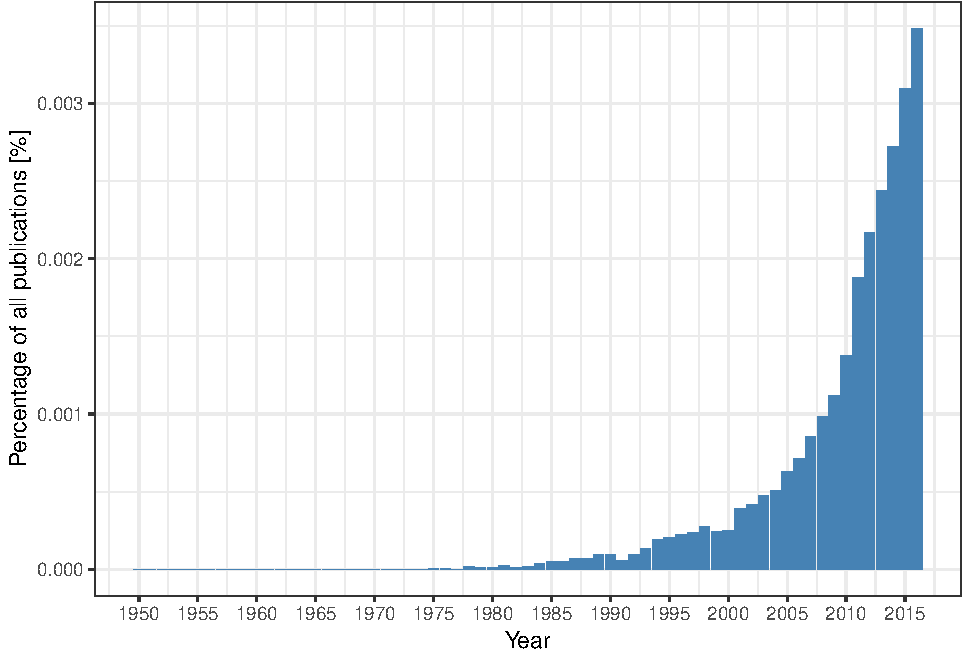
\includegraphics[width=0.7\linewidth]{UCzPhDThesis_files/figure-latex/pubmedTME-1} 

}

\caption{Percentage of publications containg phrase
``tumor immunotherapy'' is growing, numbers retreived on 17.01.2017 from
\href{http://dan.corlan.net/medline-trend.html}{Medline Trends}
\citet{REF}}\label{fig:pubmedTME}
\end{figure}






\hypertarget{tumor-micro-environment-fiend-or-foe}{%
\subsection{Tumor micro environment: fiend or
foe?}\label{tumor-micro-environment-fiend-or-foe}}

\hypertarget{what-is-tumor-microenvironment-tme}{%
\subsubsection{What is Tumor Microenvironment
(TME)}\label{what-is-tumor-microenvironment-tme}}

Tumor Microenvironment is a complex tissue that surrounds tumor cells.
It is composed of blood and lymphatics vessels, epithelial cells,
mesenchymal stem cells, fibroblast, adipocytes and a wide variety of
immune cells. Their proportion and specific roles vary significantly
with tumor type and stage. Communication between the environmental cells
and the tumor is critical for tumor development and its impact on
patient's response to treatment.

\hypertarget{tme-as-tumor-allay}{%
\subsubsection{TME as tumor allay}\label{tme-as-tumor-allay}}

In 1863 Rudolf Virchow observed a link between chronic inflammation and
tumorigenesis. Accoriding to Virchov theory genetic damage would be the
``match that lights the fire'' of cancer, and the inflammation or
cytokines produced by immune cells should be the ``fuel that feeds the
flames''. (\citet{Inflammation} and cancer: back to Virchow?). Therefore
lymphocyte infiltration was confirmed by subsequent studies as a
hallmark o cancer. The question one may ask is why our immune system
does not defend the organism from tumor cells as it does in a range of
bacterial and viral infections? It is mainly because of the ability of
tumor cells to inhibit immune response through activation of negative
regulatory pathways (so called immune checkpoints).

Many examples can be cited on how TME facilitates tumor development. For
instance, in the early stages of tumorigenesis some macrophage
phenotypes support tumor growth. Also, it was shown that myeloid-derived
suppressor cells (MDSCs) have an ability to suppress immune defence
i.e.~immunosurveillance by dendritic cells (DCs), T cell activation and
macrophage polarisation and they promote tumor vascularisation as well.
(@ Talmadge, J.E. \& Gabrilovich, D.I. History of myeloid-derived
suppressor cells. Nat. Rev.~Cancer 13, 739--752 (2013).44. @
Gabrilovich, D.I., Ostrand-Rosenberg, S. \& Bronte, V. Coordinated
regulation of myeloid cells by tumours. Nat. Rev.~Immunol. 12, 253--268
(2012). Tregs and myeloid-derived suppressor cells can negatively impact
natural immune defence and by these means allow growth and invasion of
tumor cells. (\citet{Implications} of the tumor immune microenvironment
for staging and therapeutics Janis M Taube1,2,3, Jérôme Galon). Another
cell type, a part of ECM, fibroblast, or more precisely Cancer
Associated Fibroblasts (CAFs) have proven pro-tumor functions in breast
cancer where they enhance metastasis. (@ Dumont, N. et al.~Breast
fibroblasts modulate early dissemination, tumorigenesis, and metastasis
through alteration of extracellular matrix characteristics. Neoplasia
15, 249--262 (2013).)

In addition, it is worth mentioning the role of ECM as an integral part
of TME and its impact on tumorigenesis and metastatis. It is usually
anit-tumor in early stages and pro-tumor at the metastatic stages. The
blood and lymphatic vessels maintain tumor growth providing necessary
nutritive compound to malignant cells.

HALLMARKS?

Fig 2 The micronvironment supports metastatic dissemination and
colonistaion at secondary sites ? (\citet{Microenvironmental} regulation
of tumor progression and metastasis)

\hypertarget{two-faced-nature-of-immune-cells}{%
\subsubsection{Two-faced nature of immune
cells}\label{two-faced-nature-of-immune-cells}}

Recent studies unveil ambivalent nature of immune cells of TME. While
some as cytotoxic T cells, B cells and macrophages can manage to
eliminate tumor cells. Treg cells role is to regulate expansion and
activation of T and B cells. Depending on cancer type, they can be
either pro- or anit- tumor. For example as it has been shown for Tregs,
they can be also associated with improved survival (i.e.~in colorectal
cancer(@. Frey, D.M. et al.~High frequency of tumor-infiltrating FOXP3+
regulatory T cells predicts improved survival in mismatch
repair-proficient colorectal cancer patients. Int. J. Cancer 126,
2635--2643 (2010).). For innate immunity, there are widely accepted M1
(ani-tumor) and M2 (pro-tumor) extreme macrophages phenotypes in TME.
(\citet{Qian}, B.Z. \& Pollard, J.W. Macrophage diversity enhances tumor
progression and metastasis. Cell 141, 39--51 (2010). Most of the
statements seem to be context dependent and not valid universally across
all cancer types. We already mentioned Macrophages phenotypic plasticity
as well as different behaviour of EMC depending on tumor stage.

From more general point of view, it has been observed that
immunodeficiency can correlate with high cancer incidence. Results of
analysis based on observations of 25,914 female immunosuppressed organ
transplant recipients, the tumor incidence was higher than predicted for
multiple cancers. However, the number of breast cancer cases decreased
which can be really disturbing if we need to decide on the role of
immune defence in tumor progression (\citet{Stewart} T., Tsai, S.C.,
Grayson, H., Henderson, R. \& Opelz, G. Incidence of de-novo breast
cancer in women chronically immunosuppressed after organ
transplantation. Lancet 34, 796--798 (1995).) This trend was confirmed
through a study on individuals with AIDS and other studies. This
indicates that immune microenvironment can be cancer stimulating or
inhibiting depending on the type of cancer.

\begin{itemize}
\tightlist
\item
  review hallmarks of cancer immune
\end{itemize}

\hypertarget{cancer-immune-phenotypes}{%
\subsection{Cancer immune phenotypes}\label{cancer-immune-phenotypes}}

There can be distinguished cancer phenotypes depending on immune
infiltration how they are measured, defined, indexes, types of cancer,
impact

\begin{quote}
In further support of a role for memory T cells in antitumour responses,
tumour-infiltrating lymphocytes that express CD4 or CD8 extracted from
experimental tumour models typically have the features of memory T cells
and can possess an activated or exhausted phenotype, expressing markers
such as PD-1, T-cell immunoglobulin and mucin-domain containing protein
3 (TIM-3) and lymphocyte activation gene 3 (LAG-3). (\citet{IMMUNE}
CANCER CIRCLE)
\end{quote}

\begin{quote}
Anticancer immunity in humans can be segregated into three main
phenotypes: the immune-desert phenotype (brown), the immune--excluded
phenotype (blue) and the inflamed phenotype (red). (\citet{IMMUNE}
CANCER CIRCLE Fig 3)

Inflamed versus non-inflamed tumours

What is the basis for the three immune profiles observed in tumours? To
a first approximation, differences between the profiles can be ascribed
to whether tumours harbour an inflammatory microen-vironment, which can
reflect variations in a number of cellular and other factors (Fig.~4).
The degree of inflammation can be gauged by the cellular content of the
tumour~---~for example, the presence of immune cells, either in the
parenchyma or at the invasive margin of the tumour78,79. Inflamed
tumours also contain proinflammatory cytokines that should provide a
more favourable environment for T-cell activa-tion and expansion,
including type~I and type~II IFNs, IL-12, IL-23, IL-1β, tumour-necrosis
factor (TNF)-α and IL-2. However, it is unclear whether the presence of
these cytokines is the cause or consequence of the cellular influx. The
production of tropic chemokines by lympho-cytes and myeloid cells is
therefore likely to be an important feature of inflamed
tumours.Non-inflamed tumours generally express cytokines that are
associ-ated with immune suppression or tolerance. They can also contain
cell types associated with immune suppression or tissue homeostasis. As
well as regulatory T~cells, these cells include the lesser characterized
populations of myeloid-derived suppressor cells (for example, immature
granulocytes) and tumour-associated macrophages, which are unacti-vated
and often called M2~macrophages. However, regulatory T~cells are not
associated uniquely with non-inflamed tumours as they typically
accompany effector T~cells into inflammatory sites and are important for
maintaining immune homeostasis, even in the presence of an active
antitumour immune response
\end{quote}

immunoscore

immunophenoscore

ML based scoring scheme. Random forest

link to \emph{precision medecine}

\begin{quote}
Together, these observations support the notion that gene
expression-based correlates of immune involve- ment could hold valuable
clinical utility for a number of prognostic and therapy-predictive
applications. However, to date, mRNA-based diagnostics that quantify
immune involvement in tumors do not exist. Multi-gene diagnos- tics that
simultaneously measure mRNA transcripts of multiple genes represent a
class of In Vitro Diagnostic Multivariate Index Assay (IVDMIA) that has
in recent years gained wide clinical acceptance for the diagnosis and
stratification of patients into risk groups to guide therapeutic
decisions {[}80, 81{]}
\end{quote}

\begin{quote}
These observations raise the question of the underlying molecular
mechanisms that explain the differences in immunogenicity of the tumors.
The question can be reduced to the notion of sources of immunogenic
differences, which can be divided into two categories: tumor-intrinsic
factors and tumor-extrinsic factors. Tumor-intrinsic factors include the
mutational load, the neoantigen load, the neoantigen frequency, the
expression of immunoinhibitors and immunostimulators (e.g., PD-L1), and
HLA class I molecule alterations. Tumor-extrinsic factors include
chemokines that regulate T cell trafficking, infiltration of effector
TILs and immunosuppressive TILs, and soluble immunomodulatory factors
(cytokines) (\citet{Gajewski} et al., 2006Immune resistance orchestrated
by the tumor microenvironment.)

For each of the studied cancers, the analysis revealed only
immune-related factors, which we classified into four categories: (1)
infiltration of activated CD8+/CD4+ T cells and Tem CD8+/CD4+ cells; (2)
infiltration of immunosuppressive cells (Tregs and MDSCs); (3)
expression of MHC class I, class II, and non-classical molecules; and
(4) expression of certain co-inhibitory and co-stimulatory molecules
(\href{http://www.cell.com/cms/attachment/2109515464/2082923785/gr5.jpg}{Figure
5}A).To visualize the information, we constructed an immunophenogram
that includes these four categories
(\href{http://www.cell.com/cms/attachment/2109515464/2082923785/gr5.jpg}{Figure
5}B). We then calculated an aggregated score, immunophenoscore, based on
the expression of the representative genes or gene sets comprising four
categories: MHC molecules, immunomodulators, effector cells (activated
CD8+ T cells and CD4+ T cells, Tem CD8+ and Tem CD4+ cells), and
suppressor cells (Tregs and MDSCs) Multivariate analysis showed that the
immunophenoscore was associated with survival in 12 solid cancers, of
which 4 were significant: KIRC, SKCM, breast cancer (BRCA), and bladder
cancer (BLCA)
(\href{http://www.cell.com/cms/attachment/2109515464/2082923785/gr5.jpg}{Figure
5}C).

The immunophenoscore we developed was derived in an unbiased manner
using the TCGA data and machine learning, but it reflects current
understanding of the categories of genes that determine immunogenicity
of the tumors: effector cells, immunosuppressive cells, MHC molecules,
and immunomodulators. The immunophenoscore is similar to the conceptual
immunogram that was recently proposed to represent the status of the
immune system (\href{javascript:void(0);}{Blank et al., 2016}). Another
advantage of the immunophenoscore is that it represents a standardized
value because \emph{Z} scores are used, and is therefore more robust
compared with the use of expression values. However, because presently
only limited data are available, additional studies are required to
validate the immunophenoscore. Notably, the method can be further
improved by optimizing the immunophenoscore for specific cancers.
Finally, for routine applications, other techniques for gene expression
profiling like microarrays and qPCR can be used instead of
RNA-sequencing.
\end{quote}

\hypertarget{immune-signatures}{%
\subsection{Immune signatures}\label{immune-signatures}}

definition of signature: marker genes, list of genes, weighted list we
can talk about the general immune signature of signature of immune
infiltration and stroma or immune signature of a specific cell type of
functional subpopulation purpose of signatures

availability of immune signatures

the problem of not consistency of immune signatures origin of signatures

``the gene expression profiles of tumour-associated immune cells differ
considerably from those of blood derived immune cells''(\citet{Shelker}
et al.~Estimation of immune cell content using single cell data)

\hypertarget{immunotherapies}{%
\section{Immunotherapies}\label{immunotherapies}}

This section outlines progress in cancer therapies with a focus on
immune therapies. It will link the ongoing research on TME with
therapeutical potential.

\hypertarget{cancer_Therapies}{%
\subsection{Cancer therapies}\label{cancer_Therapies}}

\hypertarget{recent-progress-in-immuno-therapies}{%
\subsection{Recent progress in
immuno-therapies}\label{recent-progress-in-immuno-therapies}}

The immunotherapies, in contrast with other types of cancers therapies
discussed in \protect\hyperlink{cancer_Therapies}{the previous chapter},
aim to trigger or restart the immune system to defend the organism and
attack the malignant cells. All this, however without provoking
persisting inflammation state (\citet{Predina}, J., (2013). Changes in
the local tumor microenvironment in recurrent cancers may explain the
failure of vaccines after surgery. Proc. Natl. Acad. Sci. USA 110,
E415--E424.)

The idea of stimulating immune system to fight malignant cell was not
born recently. Since a long time a possibility of development of an
anti-cancer vaccine has been investigated. Unfortunately, this idea
faced two important limitations 1) lack of knowledge of antigens that
should be used in vaccine to successfully stimulate cytotoxic T cells 2)
the ability of cancer to block the immune response also called
\emph{immunostat}. Despite those impediments works on anti-tumor
vaccines do not cede. (\citet{Palucka}, K., and Banchereau, J. (2013).
Dendritic-cell-based therapeutic can- cer vaccines. Immunity 39, this
issue, 38--48.)

Another idea involving using immune system as a weapon to fight cancer,
would be the use of genetically modified patient's T-cells, carrying
\emph{CARs} (chimeric antigen receptors) (\citet{Jackson} Driving CAR
T-cells forward nat rev 2016). After a long period of small unsuccessful
trials, recently in 2017, two CAR T-cell therapies were accepted, one to
``treat adults with certain type of large B-cell lymphoma''
(\citet{FDA_CAR-T_adult}), other to treat ``children with acute
lymphoblastic leukemia (ALL)'' (\citet{FDA_CAR-T_ALL}) , which are, at
the same time, the first two gene therapies accepted by FDA.

However, the two most promising immuno-related strategies are based on
blocking so called immune check point inhibitors: cytotoxic T-lymphocyte
protein 4 (CTLA4) and programmed cell death protein 1 (PD-1). The
anti-CLTA4 antibodies blocks repressive action of CLTA4 on T-cells and
they become therefore activated. It was shown efficient in melanoma
patients and accepted by FDA in 2015 as adjuvant therapy for stage III
metastatic melanoma patients (\citet{FDA_CTLA4}). PD-1 is a cell surface
receptor of T cells, that binds to PD-L1/PD-L2. After binding, an
immunosuppressive pathway is activated and T cells activity is dampened.
An action of an anti-PD-L1 antibody is to prevent this immune
exhaustion.(\citet{IMMUNE} CANCER CIRCLE). A stepping stone for
anti-PD-L1 therapies was approval of Tecentriq (atezolizumab) for
Bladder cancer (\citet{FDA_PDL1_Bladder}) and anit-PD1 Keytruda
(pembrolizumab) initially accepted for NSCLC and further extended to
head and neck cancer, Hodgkin's lymphoma, gastric cancer and
microsatellite instability-high cancer (\citet{FDA_PDL1_NSCLC}). Since
other anti-PD-L1 or anti-PD1 antibodies were accepted or entered
advanced stages of clinical trials (\citet{Wolchok}, 2015,PD-1
blockers). A short history of immunotherapy FDA-accepted treatments can
be found in Fig. \ref{fig:timeline-immunotherapies}

\begin{figure}

{\centering 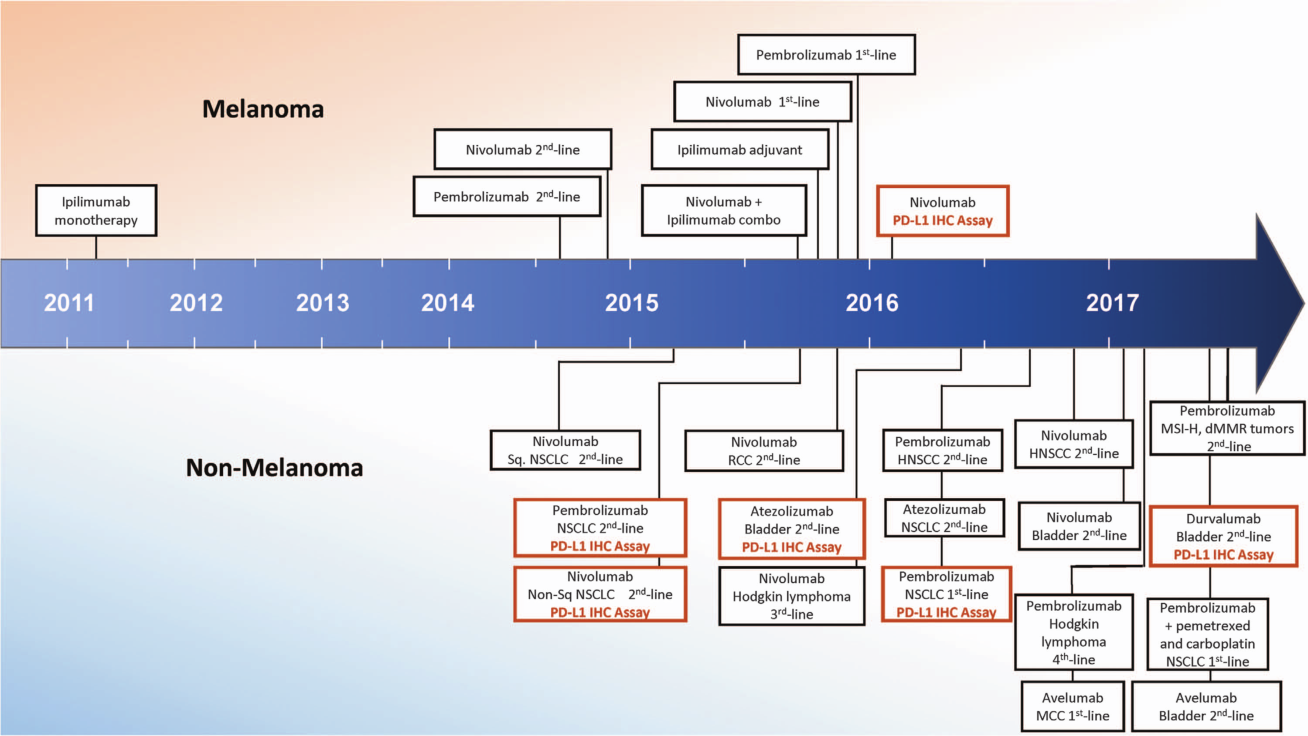
\includegraphics[width=1\linewidth]{figures-ext/02-timeline-immunotherapies} 

}

\caption{This timeline describes short
history of FDA approval of checkpoint blocking immunotherapies up to
2017. Reprinted by permission from Springer Nature,
(\citet{Implications} of the tumor immune microenvironment for staging
and therapeutics Janis M Taube1,2,3, Jérôme Galon), © 2017 Macmillan
Publishers Limited, part of Springer Nature. All Rights Reserved.}\label{fig:timeline-immunotherapies}
\end{figure}








The main drawback of immunotherapies is a heterogeneity of response
rate, which can vary i.e.~from 10--40\% in case of PD-L1blocking(@ Zou,
W., Wolchok, J. D. \& Chen, L. PD-L1 (B7-H1) and PD-1 pathway blockade
for cancer therapy: mechanisms, response biomarkers, and combinations
Sci. Transl. Med. 8, 328rv4 (2016).) , suggesting that some patient can
have more chances than others to respond to an immune therapy. So far,
it has been shown that anti PD-L1 therapies works more effectively in T
cell infiltrated tumors with exclusion of Tregs because of lack of
difference in expression of FOXP3 in responding and non-responding group
of patients. (\citet{Herbst.predictive} role PD\_L1\_. Also some light
has been shade by Rizvi et al (@. Rizvi, N. A.et al.~Mutational
landscape determines sensitivity to PD-1 blockade in non-small cell lung
cancer. Science 348, 124--128 (2015). who connected mutational rate of
cancer cells to the chances of response to an immunotherapy.

Despite those fundings, the precise qualifications of patients that
should be sensitive to an immunotherapy are not defined (\citet{Pitt} et
al., 2016,Resistance mechanisms to immune-checkpoint blockade in cancer:
tumor-intrinsic and -extrinsic factors.). As most patients do not answer
to immunotherapies, it stimulates researches to look for better
biomarkers and patient stratifications, and pharmaceutical industries to
discover new immune checkpoints based therapies.

\hypertarget{potential-of-development-of-new-immunotherapies}{%
\subsection{Potential of development of new
immunotherapies}\label{potential-of-development-of-new-immunotherapies}}

?

\hypertarget{quantifying-immune-infiltration-data}{%
\section{Quantifying immune infiltration
(data)}\label{quantifying-immune-infiltration-data}}

Nowadays, more and more biological data is produced. However, this
proliferation of accessible resources is not proportional to generated
insights and wisdom. In this thesis, we wok mostly generate
\emph{Knowledge} and \emph{Insights} and we hope to generate some
\emph{Wisdom} (Fig. \ref{fig:information-power}). However, in this part,
we will introduce the foundation of our analysis: different data types
that will be further discussed in chapters that follow.

\begin{figure}

{\centering 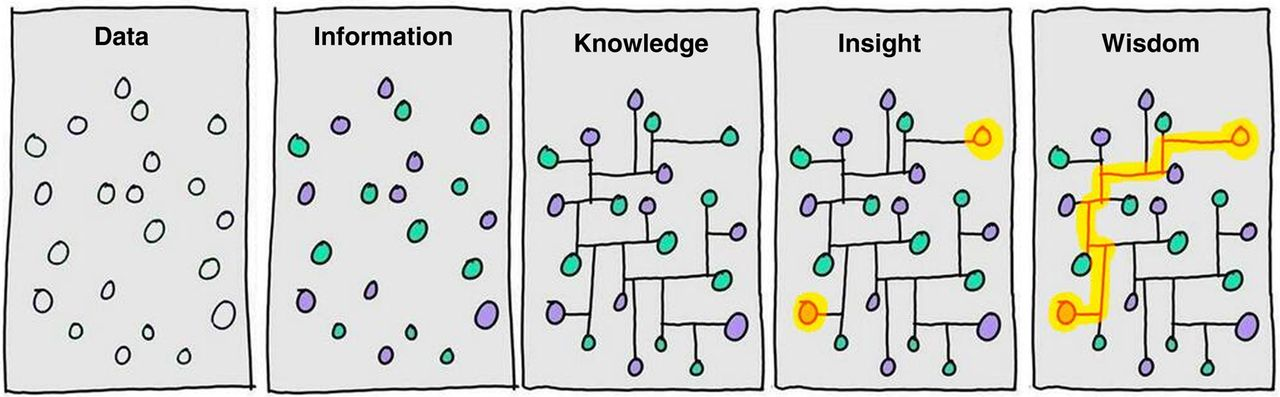
\includegraphics[width=0.8\linewidth]{figures-ext/01-Information_power} 

}

\caption{\textbf{From \emph{Data} to
\emph{Wisdom}}. Illustration of different steps that it takes to go from
\emph{Data} to generating \emph{Wisdom}. It highlights that generating
data is not equal to understanding it and additional efforts are needed
to generate value. Image authored by Clifford Stoll and Gary Schubert
published by Portland Press Limited on behalf of the Biochemical Society
and the Royal Society of Biology and distributed under the
\href{https://creativecommons.org/licenses/by/4.0/}{Creative Commons
Attribution License 4.0 (CC-BY)} in (\citet{BIG}
DATAOMICShttp://www.emergtoplifesci.org/content/1/3/245.article-info).}\label{fig:information-power}
\end{figure}












We will introduce most relevant data types that are used to study immune
infiltration of tumors.

\hypertarget{facs}{%
\subsection{Facs}\label{facs}}

\begin{quote}
Flow cytometry : Laser-based technology that allows for simultaneous
quantification of the abundance of up to 17 cell surface proteins using
fluorescently labelled antibodies. (\citet{Single-cell} RNA sequencing
to explore immune cell heterogeneity) cost : 0.05\$/ cell
\end{quote}

\begin{quote}
Mass cytometry(commercial name CyTOF). Mass spectrometry technique used
as an alternative to flow cytometry that allows for the quantification
of cellular protein levels by using isotopes that overcome problems
associated with the spectral overlap of fluorophores. 40 prot per cell
(\citet{Single-cell} RNA sequencing to explore immune cell
heterogeneity) 35\$/cell
\end{quote}

\hypertarget{staining}{%
\subsection{staining (histopathology, immunoscore!!! , multiplex
immunofluorescence)}\label{staining}}

\begin{quote}
The standardized Immunoscore was based on the quantification (cells/mm2)
of two lymphocyte populations (CD3 and CD8) within the central region
and the invasive margin of colorectal carcinoma tumors and provides a
scoring system ranging from Immunoscore 0 (I0) to Immunoscore 4 (I4)
(Figure 4).41 (\citet{Implications} of the tumor immune microenvironment
for staging and therapeutics Janis M Taube1,2,3, Jérôme Galon)
\end{quote}

\begin{quote}
The immune cell content of a tumour sample can also be determined by
using more established multiplexed methods like immunohistochemistry
(IHC) or immunofluorescence (IF)20 or newer methods like imaging mass
cytometry using FFPE tissue samples21. The advantage of these techniques
is that a larger number of cells can be analysed and that these
techniques also provide information about the spatial distribution of
the different cell types. However, these methods are limited to the
number of proteins that can be analysed simultaneously currently
(ranging from \textasciitilde{}10 to 100), advantage of the
deconvolution approach is that it is unbiased (i.e., hypothetical
response markers do not need to be pre-specified). It allows one to link
both the cellular characteristics and the cellular content with
treatment response. We anticipate that this approach will aid in the
discovery of novel predictive response biomarkers for both conventional
and immune-directed therapy by taking cellular composition into account.
(\citet{Shelker} et al.~Estimation of immune cell content using single
cell data).
\end{quote}

\hypertarget{omics}{%
\subsection{omics}\label{omics}}

Some kind of sequencing explanation needed for non-biologists

\hypertarget{transcriptome}{%
\subsubsection{transcriptome}\label{transcriptome}}

\begin{quote}
Transcriptomics is the large-scale study of RNA mole- cules by use of
high-throughput techniques. It examines the abundance and makeup of a
cell's transcriptome1,2. In contrast to DNA, which is largely identical
across all cells of an organism, the actively transcribed RNA is highly
dynamic, reflecting the diversity of cell types, cellular states and
regulatory mechanisms. Because a transcrip- tome profile can be regarded
as a signature or snapshot of the underlying cell state, the
experimental profiling of samples and specimens can provide insights
into their unique biology.

Transcriptome profiling can detect changes in gene activity and
regulation by capturing quantitative expres- sion patterns and has the
capacity to describe the under- lying phenotypes in great detail.
Furthermore, many genetic and epigenetic events can be either directly
observed or indirectly inferred from transcriptomic data. The primary
readouts of modern-day cancer tran- scriptomics can be broadly
categorized as genetic and functional (FIG. 2). Whereas functional
measurements benefit mostly from the breadth of genome-wide assays, the
detection of genetic events required increased depth and base pair
resolution.

Although most transcriptomic platforms are highly reproducible by
themselves, reproducibility across platforms is limited. Unfortunately,
the biggest challenge is in the measurement of absolute expression
levels263, which is the input to many biomarkers and signatures.
Therefore, signatures cannot be expected to translate verbatim between
platforms. Few studies have explored this topic. Fumagalli et al.264
concluded that single-gene expression biomarkers and established
prognostic signatures generalize well between microarrays and RNA
sequencing (RNA-seq). Zhang et al.265 reached a similar conclusion in
that ``technological platforms (RNA-seq versus microarrays)
{[}\ldots{}{]} do not significantly affect performances of the
{[}predictive{]} models.'' However, these studies were done on
high-quality samples and did not explore whether RNA degradation or
crosslinking had a detrimental effect.

Types of gene expression analyses. Transcriptome- wide gene expression
profiles are now available for the majority of cancer types and their
corresponding tissues of origin. In general terms, there are two
cancer-centric paths to analyse these data: the differential approach,
which interprets tumour expression profiles relative to the
patient-matched or unmatched normal tissue sam- ples; and the relative
approach, which compares tran- script levels across tumours or other
samples (FIG. 3). Inherently, these strategies have unique advantages
and applications. Differential analyses are designed to detect
cancer-specific changes, but if the normal samples are not
comparable164, the results will be difficult to inter- pret, for
example, if the cancer cell of origin is rare or unknown. In general
terms, differential analyses tend to be underpowered in the clinical
setting. Comparisons at the single-patient level are often limited by
the dearth of replicates due to cost and sample availability, while at
the cohort level, they are often confounded by interpatient
heterogeneity. Relative analyses are useful to charac- terize individual
samples but typically depend on the availability of external knowledge
or reference data sets. The validity of any relative comparison is
contingent on how well a query sample is matched to the reference in
terms of technical (for example, type of data processing) and biological
(for example, molecular subtype) biases. Therefore, relative analyses
often necessitate advanced normalization techniques165 and batch
correction166. Overall, the differential approach is more common in the
research setting to generate hypotheses, whereas the relative approach
drives many clinical applications, such as precision medicine.
Differential approaches. The simplest type of differen- tial analysis is
the identification of genes that are upreg- ulated or downregulated in
cancer (that is, differentially expressed genes (DEGs)), and established
methods to detect DEGs are available for both microarray167 and RNA-seq
data168--170. A typical result is a long list of DEGs that is difficult
to interpret without additional functional annotation, as demonstrated
by a landmark study in breast cancer171. Differential methods have also
been proposed for splicing93 or isoform usage172. Although
transcriptomes have very high dimensionality, there is also substantial
correlation among the genes, which can be leveraged to simplify or
summarize the data173. A common strategy is to break down the transcrip-
tome-wide gene expression profile into a set of modules that are less
interdependent, more generalizable and simpler to understand. The
specifics for each method differ substantially, but in general, it is
possible to test for differential gene sets174, pathways, gene
regulatory networks or modules in co-expression networks175. Ideally,
testing multiple related genes will improve sen- sitivity and yield
results that are easier to understand. For example, using a simple gene
set method, Majeti et al.176 were able to identify the dysregulation of
the WNT pathway in acute myeloid leukaemia. Beyond upregulation or
downregulation, methods have been developed to detect less-uniform
changes in gene expres- sion177; for example, detecting mechanism of
action by network dysregulation (DeMAND) leverages changes in
correlation to prioritize dysregulated or `rewired' modules178

Cellular composition and microenvironment. The study of the
heterogeneous cellular composition of tumours is one of the most recent
applications of cancer tran- scriptomics. Approaches typically involve
either directly isolating and characterizing individual cells (using,
for example, single-cell sequencing) or indirectly inferring cell
compositions in silico from bulk expression data. From bulk expression
data (which are currently more readily available from clinical samples
than are sin- gle-cell data), the computational task is often referred
to as sorting, or deconvolving, the gene expression pro- file.
Deconvolution is a difficult problem that requires methodological
constraints in order to converge on plausible solutions. A large number
of algorithms have been proposed197 that make different trade-offs on
the basis of the available data and the desired output. In general, the
methods can be divided into those that use cell-type-specific gene
signatures and can be applied to a single tumour sample and those that
require multiple tumour and normal samples (matched or unmatched).
Currently, the most important applications are to esti- mate tumour
clonality and purity, which are affected by intrinsic tumour cell
heterogeneity or infiltration by stro- mal or immune cells198. For
example, in silico purification of gene expression profiles has been
applied to improve their performance in prognosis199 and
classification200. Deconvolution also provides a unique opportunity to
study the tumour microenvironment, for exam- ple, to unravel
tumour--stromal paracrine crosstalk201. In the future, single-cell
transcriptomics is bound to revolutionize our understanding of the
tumour microenvironment202, heterogeneity203 and evolution204.

The clinical utility of RNA- seq has been demonstrated by a number of
sequencing programmes where RNA-seq identified a large num- ber of
actionable genetic events221--223. Still, targeted DNA sequencing is
currently the method of choice for many clinical applications in
precision oncology. DNA is a highly stable analyte and is therefore well
suited for molecular diagnostics.

Transcriptomics in immuno-oncology. The needfor RNA-based companion
diagnostics is particu-larly acute in immuno-oncology250. Cancer
immunephenotypes were shown to broadly reflect the activityof the host
immune system and to generalize remark-ably well across cancer types.
Numerous studies haveinvestigated the association of immune
infiltrationwith survival251--253 and found significant correlationsat
the level of immune cell types, inflammation signa-tures and individual
genes. Although immune check-point inhibitors are broadly beneficial
across cancertypes, the response rates are highly variable. It
isbecoming increasingly clear that positive responses toimmunotherapy
are associated with tumour immuno-genicity and host immune
infiltration253--255. However,given the complexity of adaptive immune
responsesand the dynamic nature of tumour--immune evasion,it is
unrealistic to expect that a single gene will besufficient to accurately
predict outcomes or guidetreatment.

The clinical utility of transcriptome profiling forimmunotherapy was
demonstrated in a landmarklongitudinal study that demonstrated that
signaturesof adaptive immunity are predictive of response to immune
checkpoint blockade254. As both prognos-tic and predictive approaches
require the expressionlevels of hundreds of genes, their clinical
translationwill depend on the routine use of whole-transcrip-tome
profiling or custom-targeted panels256. We haveshown that comprehensive
immunophenotypic datacan be obtained from clinical transcriptomes and
thatthey provide unique insights into the immunologicalheterogeneity of
metastatic tumours across all majorprimary tissue types223. RNA-seq data
are also particu-larly valuable for the development of personalized
can-cer vaccines257,258, where they can be used to identifychimeric
fusion proteins that contain putative mutantepitopes245 and help in the
selection of potentiallyhighly abundant neoantigens.

The complexity of tumour--immune cell interactionsis mirrored by the
diversity of bioinformatics approachesto characterize them. Both
data-driven198 and know-ledge-driven253 approaches have been proposed to
quan-tify the overall level of tumour--immune infiltration. Inaddition,
recent methodological advances made it pos-sible to estimate cell-type
fractions from bulk tumourexpression profiles in a process referred to
as in silicocell sorting259,260, which is similar to the `purification'
ofthe tumour cell expression profiles discussed above199,200.Finally,
clonal expansion of antitumour T cells can bedetected by the presence of
somatically rearranged TCRsequences, that is, clonotypes261. An
analogous strategycan be applied to B cells and immunoglobulin
loci262.As neoantigen prediction remains a daunting problem,RNA-seq data
are useful for both the detection of pro-tein-altering genetic
aberrations and their prioritizationbased on expression levels.

(\citet{Cancer} transcriptome profiling at the juncture of clinical
translation)
\end{quote}

\begin{quote}
Bulk RNA-seq data can easily be obtained from either flash-frozen or
formalin-fixed, paraffin-embedded (FFPE) tissue samples, including both
surgically resected material and core needle biopsies. (\citet{Shelker}
et al.~Estimation of immune cell content using single cell data).
\end{quote}

\hypertarget{methylome}{%
\subsubsection{methylome}\label{methylome}}

\begin{quote}
Changes in gene expression in tumours owing to epigenetic modifi-cations
and the expression of microRNAs probably contribute directly to
determining the immune microenvironment and immunogenicity of a tumour.
Cytokine expression during T-cell development is regu-lated by
epigenetic alterations to both DNA and chromatin96. Cancer can also be
accompanied by epigenetic changes, which makes it prob-able that such
changes will influence cytokine profiles that modulate the immune
microenvironment. In fact, DNA methylation in lung-cancer cells has been
shown to reduce the expression of IL-1β97. And PD-L1 expression can be
modulated by microRNAs, with miR-200 (a repressor of
epithelial-to-mesenchymal transition) and possibly others decreasing its
expression98. Methylation of the promoter for the gene PD-L1 itself also
seems to repress PD-L1 expression; demethylation can result in
constitutive expression in tumours, especially non-small cell lung
cancer99..

Another influence on the immune profile of a tumour that has an
epigenetic mechanism involves the tissue of origin of the tumour.
Colorectal cancer tumours commonly express elevated levels of
transforming growth factor (TGF)-β100. Presumably, this reflects the
importance of the TGF-β pathway in intestinal biology and, especially,
its role in maintaining tolerance to the gut microbiota by favour-ing
the development of regulatory T~cells101. Elevated expression of TGF-β
may also contribute to the development of abundant stromal elements in
these tumours that can restrict the access of immune cells to the tumour
parenchyma, as has been demonstrated in pancreatic cancer102. Although
other factors also contribute, it is interesting to note that pancreatic
cancer and most forms of colorectal cancer (except for the mutationally
rich microsatellite-instability-high sub-group85) respond poorly to
single-agent inhibition of PD-L1/PD-1 (refs~62, 83 and~103--105).

(\citet{IMMUNE} CANCER CIRCLE)
\end{quote}

\hypertarget{single-cell}{%
\subsubsection{single cell}\label{single-cell}}

Described above methods of process DNA from hundreds of thousands of
cells simultaneously and report averaged gene expression of all cells.
In contrast, scRNA-seq technology allows getting results for each cell
individually. This is tremendous step forward enhancement of our
understanding of cell heterogeneity and opens new avenues of research
questions.

Continuous discovery of new immune subtypes has proven that cell surface
markers that are used for phenotyping by techniques like
\protect\hyperlink{facs}{FACS} and
\protect\hyperlink{staining}{immunohistochelistry} cannot capture the
full complexity. ScRNA-seq methods allow to cluster known cell types in
subpopulations based on their genetic features. (\citet{Single-cell} RNA
sequencing to explore immune cell heterogeneity). ScRNA-seq is also able
to capture particularly rare cell types as it requires much less of RNA
material (1 ng isolated from 100-1000 cells) compared to `bulk' RNA-seq
( \textasciitilde{} 1 μg of total mRNA transcripts )

\emph{new cellular states}

\begin{quote}
In summary, these studies have established that sur‑face phenotypes are
not sufficient to define cellular states in disease and have proposed
new scRNA‑seq methods to study innate immunological processes as well as
dis‑ease pathogenesis and progression at high resolution
(\citet{Single-cell} RNA sequencing to explore immune cell
heterogeneity)
\end{quote}

This new data type also brings into the field new challenges related to
data processing due to the volume, distribution, noise, and biases.
Experts highlight as the most ``problematic'' ``batch effect'' and noise
and ``dropout effect''
(\citet{https://www.nature.com/news/single-cell-sequencing-made-simple-1.22233}).
So far, there are no official standards that can be applied which makes
data comparison and post-processing even more challenging. Up to date,
there are around 70 reported tools and resources for single cell data
processing (@ GitHub, called `Awesome Single Cell'
(\href{http://go.nature.com/2rmb1hp}{go.nature.com/2rmb1hp})) .

A limited number of single-cell datasets of tumors are made publicly
available (\citet{TABLE}).

One can ask why then developing computational deconvolution of
transcriptome if we can learn relevant information from single-cell
data. Today's reality is that single cell data does not provide a
straightforward answer to the estimation of cell proportions. The
coverage is not full and sequenced single cells are not fully
representative of the true population. For instance, neutrophiles are
not found in scRNA-seq data because of they are ``difficult to isolate,
highly labile \emph{ex vivo} and therefore difficult to preserve with
current single-cell methods'' (\citet{Shelker} et al.~Estimation of
immune cell content using single cell data). In addition, a number of
patients included in published studies of range \textless{}100 cannot be
compared to thousand people cohorts sequenced with bulk transcriptome
methods. This is mostly because single cell experiments are challenging
to perform, especially in clinicsal setting as fresh samples are
needed.(\citet{Shelker} et al.~Estimation of immune cell content using
single cell data). Today, single cell technology brings very interesting
``zoom in'' perspective, but it would be incautious to make fundings
from a restricted group of individuals universal to the whole
population. Major brake to the use of single cell technology more
broadly might be as well the price that is neatly 10x higher for single
cell sample compared to bulk
(\citet{https://www.cedars-sinai.edu/Research/Research-Cores/Genomics-Core/Documents/Single-Cell-Genomics-Pricing}---June-2017.pdf).**
(A table? )**

\begin{longtable}[]{@{}cc@{}}
\toprule
Technology & Price per sample\tabularnewline
\midrule
\endhead
scRNA-seq & 3000 \$\tabularnewline
RNA-seq & 200 \$\tabularnewline
\bottomrule
\end{longtable}

In this work, we are using single cell data in two ways. Firstly, in
\protect\hyperlink{results}{Comparative\ldots{} chapter} we compare
immune cell profiles defined by scRNA-seq, blood and blind deconvolution
(problem introduced in \protect\hyperlink{immune-signatures}{Immune
signatures section}). Secondly, in \protect\hyperlink{map}{Heterogeneity
of immune\ldots{}} we use single call data of Metastatic melanoma
generated by Tirosh et al. (\citet{Tirosh} Melanoma sc) to demonstrate
subpopulations of Macrophages and NK cells.

\hypertarget{methods}{%
\chapter{Mathematical foundation of cell-type deconvolution of
biological data}\label{methods}}

In this chapter, we will discuss how mathematical models can be used to
extract information about specific cell-types from `bulk' data or how to
unmix mixed sources. It will introduce you to basic concepts of data
analysis as well as most popular advanced solutions adapted for
estimating presence and proportion of immune cells within cancer
biopsies.

\hypertarget{introduction-to-supervised-and-unsupervised-learning}{%
\section{Introduction to supervised and unsupervised
learning}\label{introduction-to-supervised-and-unsupervised-learning}}

\hypertarget{blind-source-sepration}{%
\section{Blind source sepration}\label{blind-source-sepration}}

(ICA, NMF etc)

\hypertarget{finding-optimal-number-of-components-and-over-decomposition-of-transcriptopmes}{%
\section{Finding optimal number of components and over-decomposition of
transcriptopmes}\label{finding-optimal-number-of-components-and-over-decomposition-of-transcriptopmes}}

(adapted from BMC article)
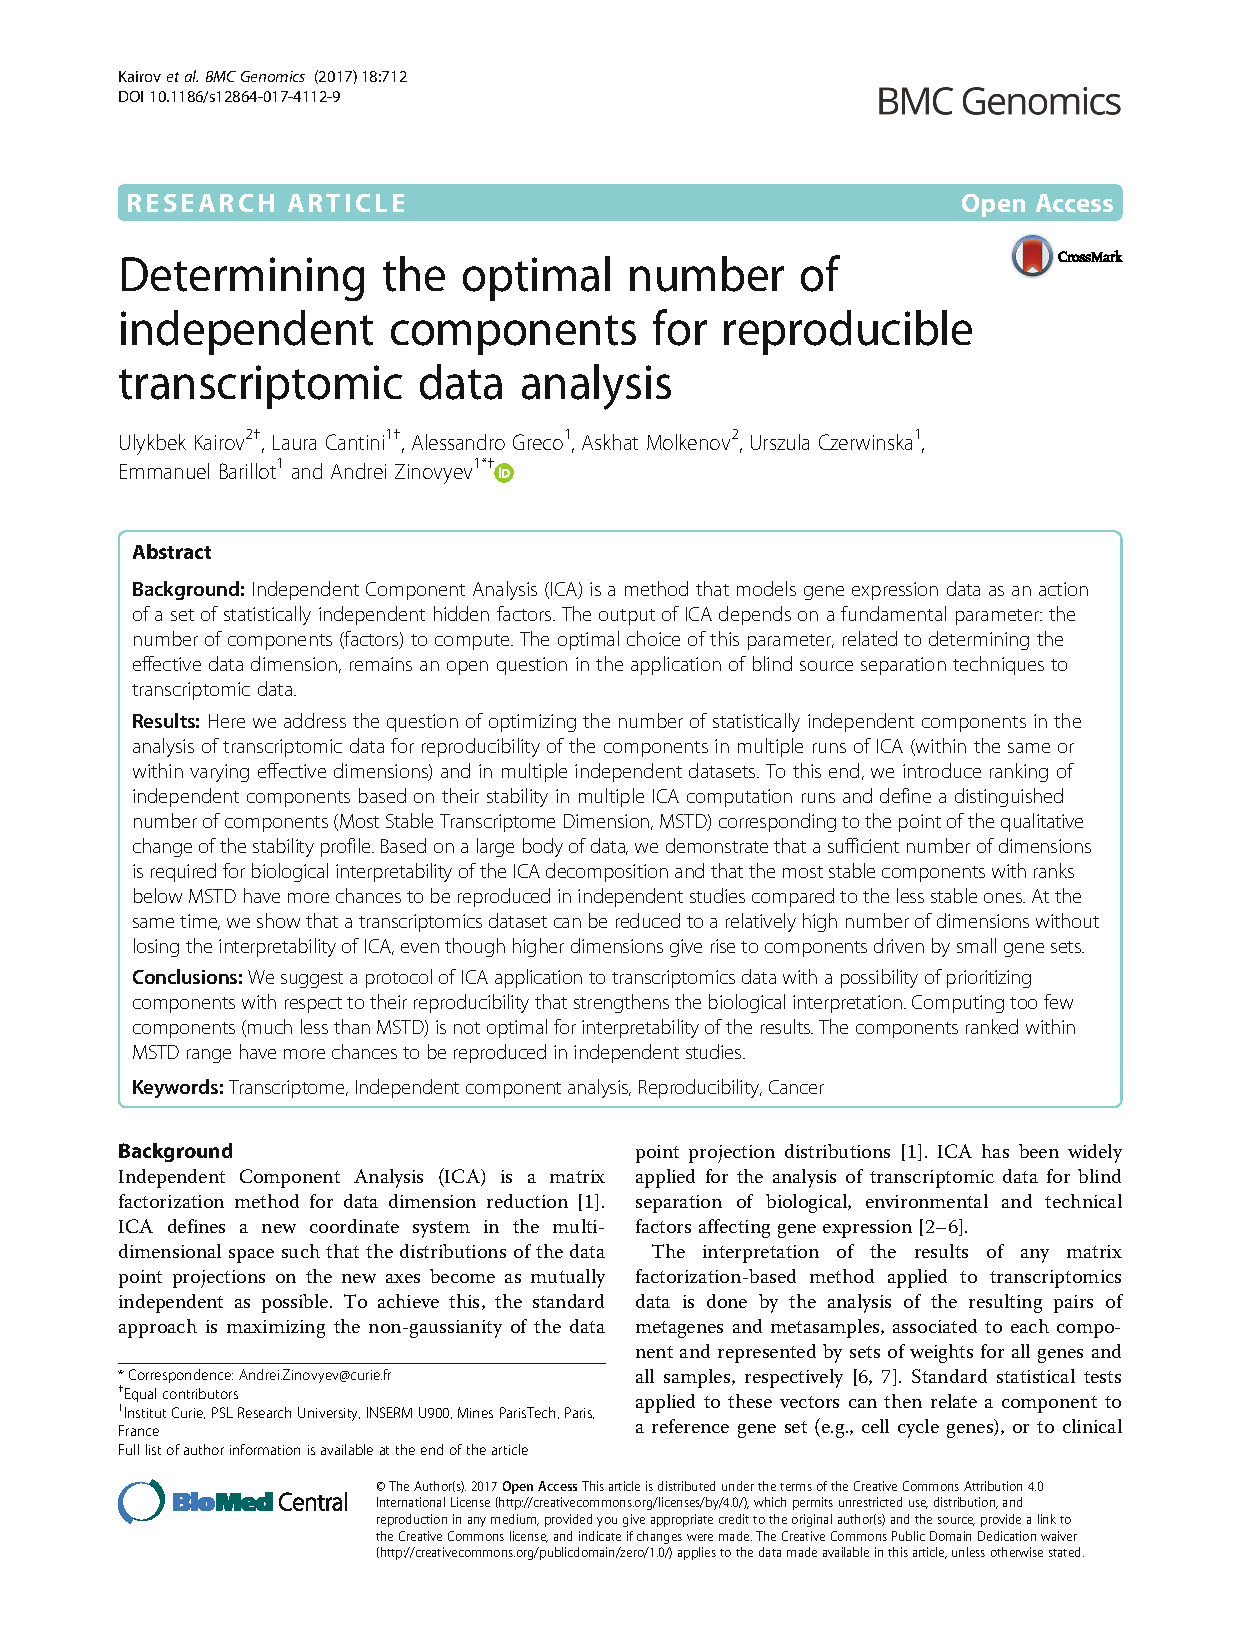
\includepdf[pages={1-}, scale=1]{pdf-ext/BMCMSTD.pdf}

\hypertarget{cell-type-deconvolution-models}{%
\section{Cell-type deconvolution
models}\label{cell-type-deconvolution-models}}

(families of approaches)

\hypertarget{basis-matrix}{%
\subsection{basis matrix}\label{basis-matrix}}

\hypertarget{regression-algorithm}{%
\subsection{regression algorithm}\label{regression-algorithm}}

\hypertarget{others}{%
\subsection{others}\label{others}}

\hypertarget{short-review-of-most-popular-cell-type-deconvolution-tools}{%
\section{Short review of most popular cell-type deconvolution
tools}\label{short-review-of-most-popular-cell-type-deconvolution-tools}}

tools will already be mentioned in the section above. However a comment
on other than mentionned aspects are needed

\hypertarget{study-of-sensitivity-of-known-methods}{%
\chapter{Study of sensitivity of known
methods}\label{study-of-sensitivity-of-known-methods}}

\hypertarget{reproducibility-of-nmf-versus-ica}{%
\section{Reproducibility of NMF versus
ICA}\label{reproducibility-of-nmf-versus-ica}}

\hypertarget{impact-of-modification-of-signatures-list-on-result-for-signature-based-deconvolution-methods}{%
\section{Impact of modification of signatures list on result for
signature-based deconvolution
methods}\label{impact-of-modification-of-signatures-list-on-result-for-signature-based-deconvolution-methods}}

\hypertarget{deconvolution-of-transcriptomes-and-methylomes}{%
\chapter{Deconvolution of transcriptomes and
methylomes}\label{deconvolution-of-transcriptomes-and-methylomes}}

We describe our methods in this chapter. The pre-eliminary pipeline and
simple results are described in the manuscript submitted to
Springer-Verlag's Lecture Notes in Computer Science
(\href{http://www.springer.com/gb/computer-science/lncs}{LNCS}) entitled
\textbf{Application of Independent Component Analysis to Tumor
Transcriptomes Reveals Specific And Reproducible Immune-related Signals}
that is placed at the end of this chapter. In the final thesis final
pipeline will be split into following structure

\hypertarget{from-blind-deconvolution-to-cell-type-quantification-general-overview}{%
\section{From blind deconvolution to cell-type quantification: general
overview}\label{from-blind-deconvolution-to-cell-type-quantification-general-overview}}

\hypertarget{the-ica-based-deconvolution-of-transcriptomes}{%
\subsection{The ICA-based deconvolution of
Transcriptomes}\label{the-ica-based-deconvolution-of-transcriptomes}}

\hypertarget{interpretation-of-independent-components}{%
\subsection{Interpretation of Independent
components}\label{interpretation-of-independent-components}}

\hypertarget{correlation-based-identification-of-confunding-factors}{%
\subsubsection{Correlation based identification of confunding
factors}\label{correlation-based-identification-of-confunding-factors}}

\hypertarget{identification-of-immune-cell-types-with-enrichment-test}{%
\subsubsection{Identification of immune cell types with enrichment
test}\label{identification-of-immune-cell-types-with-enrichment-test}}

\hypertarget{transforming-metagenes-into-signature-matrix}{%
\subsection{Transforming metagenes into signature
matrix}\label{transforming-metagenes-into-signature-matrix}}

\hypertarget{regression-based-estimation-of-cell-type-proportions}{%
\subsection{Regression-based estimation of cell-type
proportions}\label{regression-based-estimation-of-cell-type-proportions}}

\hypertarget{deconica-r-package-for-ica-based-deconvolution}{%
\section{\texorpdfstring{\emph{DeconICA} R package for ICA-based
deconvolution}{DeconICA R package for ICA-based deconvolution}}\label{deconica-r-package-for-ica-based-deconvolution}}

This part of the chapter will be adapted from package vignettes

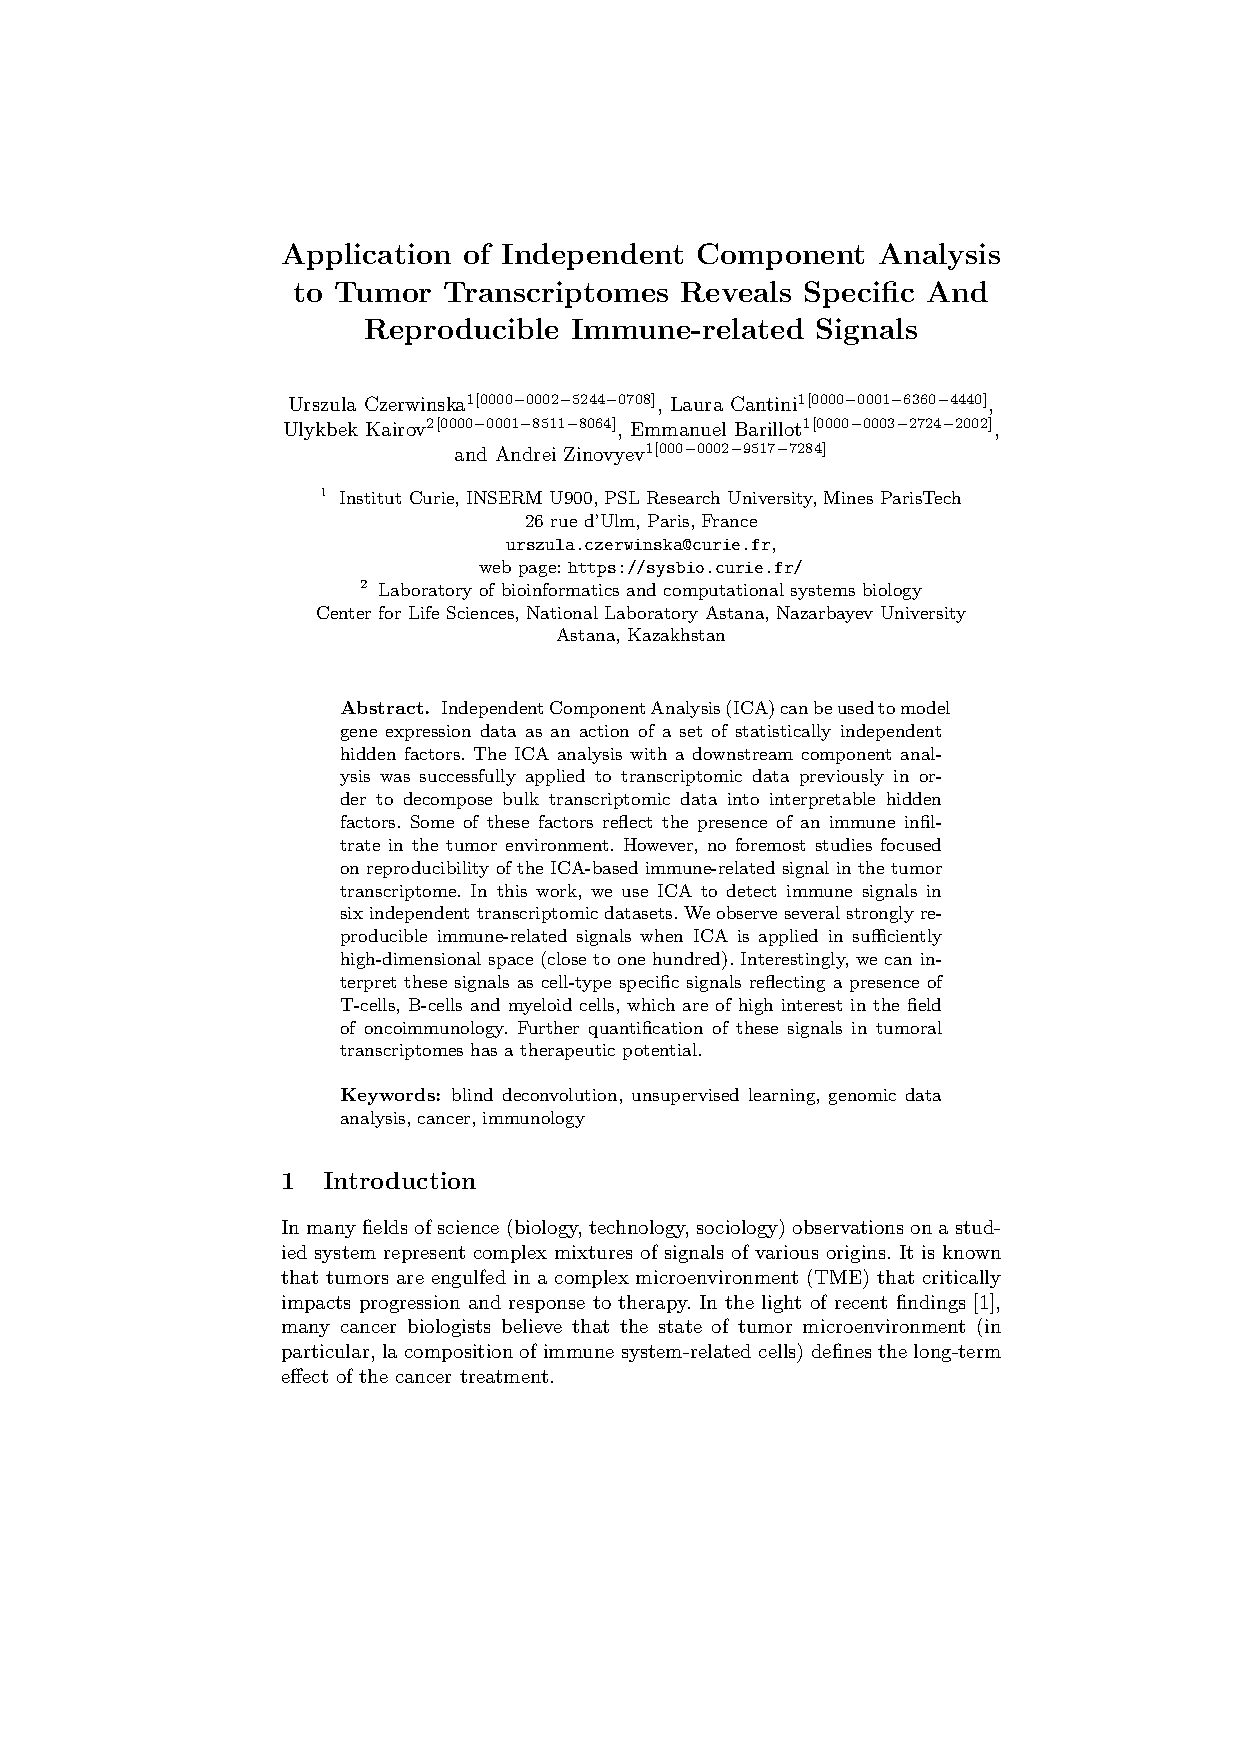
\includepdf[pages={1-}, scale=1]{pdf-ext/LVAICA.pdf}

\hypertarget{results}{%
\chapter{Comparative analysis of cancer immune
infiltration}\label{results}}

This chapter will include biological interpretation of Pan-cancer
analysis with DeconICA

\hypertarget{section}{%
\section{}\label{section}}

\hypertarget{map}{%
\chapter{Heterogeneity of immune cell types}\label{map}}

Adapted from \emph{submitted} article of Kondratova et al.

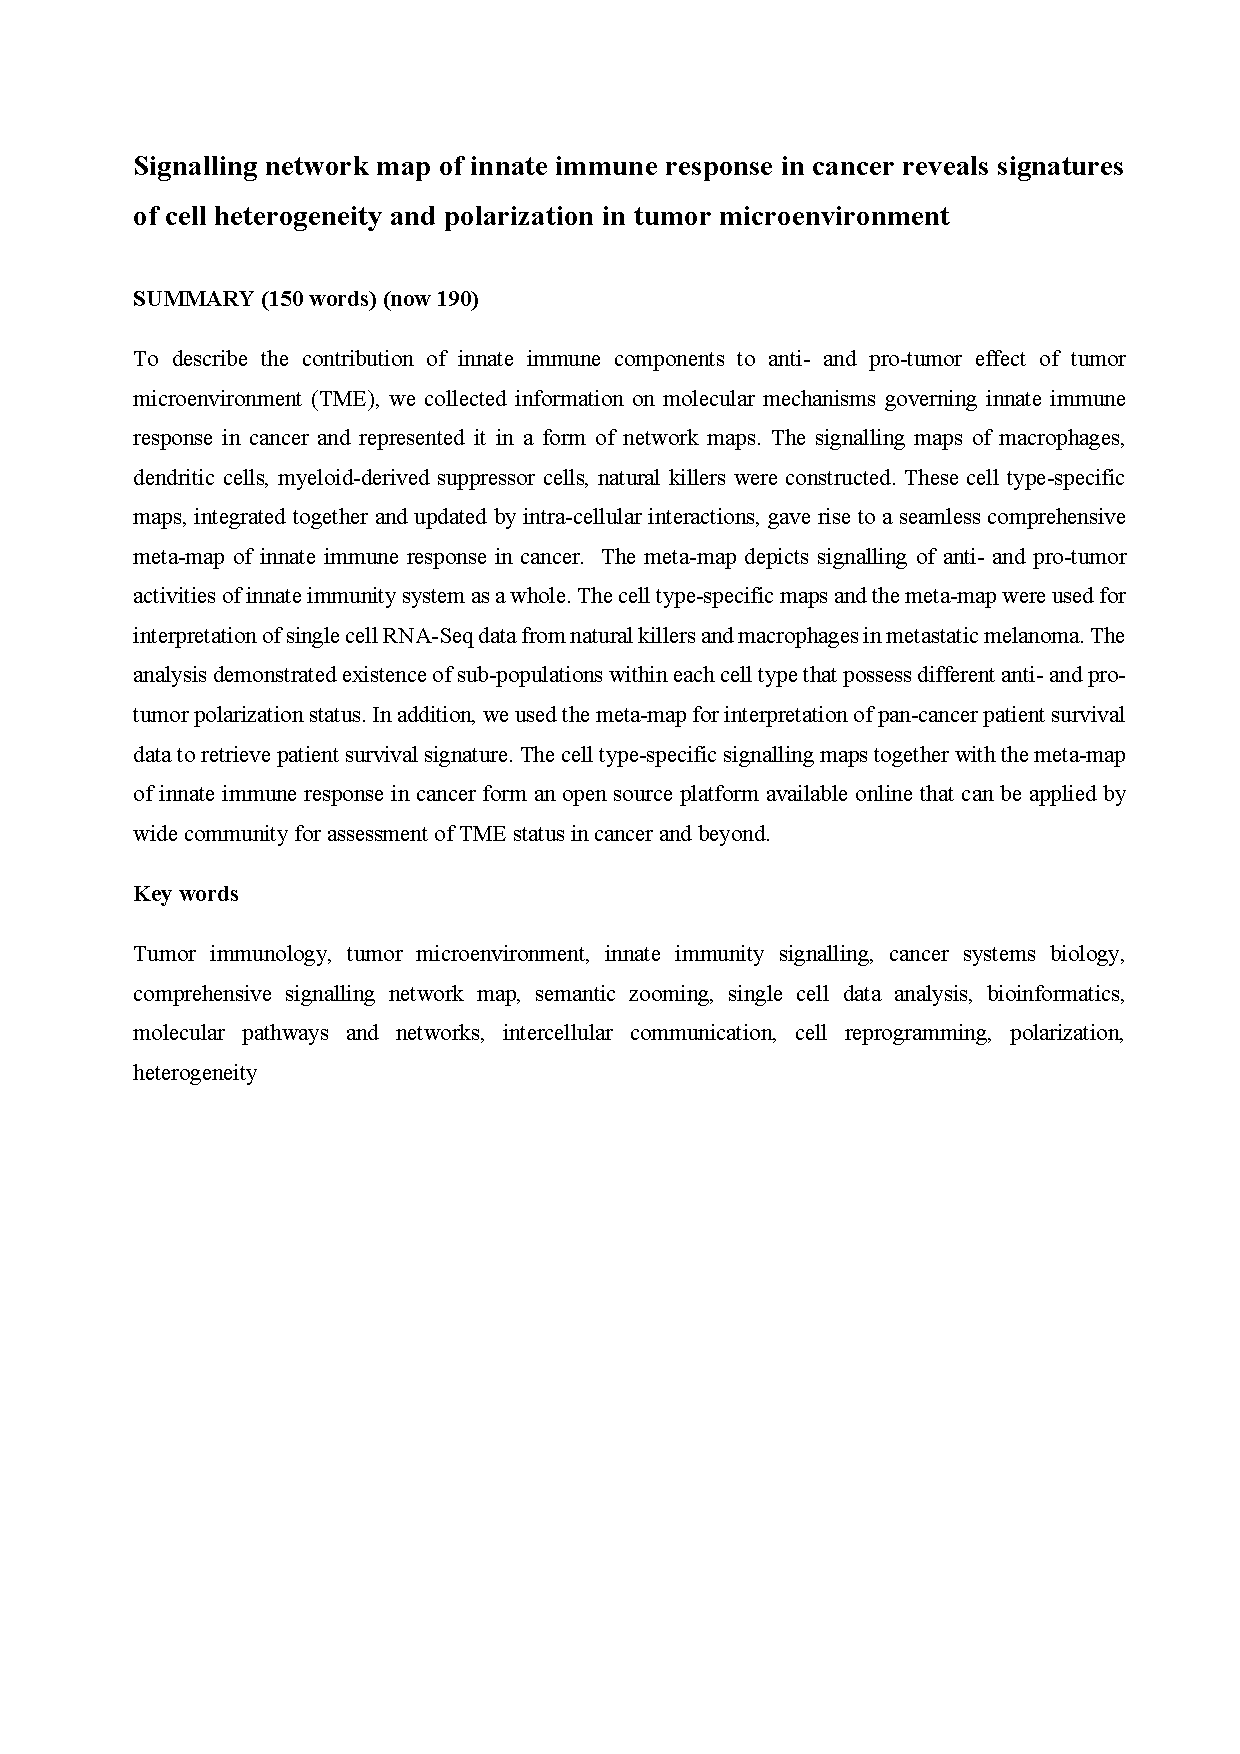
\includepdf[scale=1]{pdf-ext/ImmuneMap.pdf}

\hypertarget{annexes}{%
\chapter*{Annexes}\label{annexes}}
\addcontentsline{toc}{chapter}{Annexes}

\emph{Note: This annexes will not be a part of final manuscript}

\hypertarget{phd-timeline-for-defence-before-the-end-of-october-2018}{%
\section*{PhD timeline for defence before the end of October
2018}\label{phd-timeline-for-defence-before-the-end-of-october-2018}}
\addcontentsline{toc}{section}{PhD timeline for defence before the end
of October 2018}

In order to defend before 31 October, I need to follow the guidelines of
the University.

\begin{itemize}
\tightlist
\item
  \textasciitilde{}29 June - officially submlit the jury proposal and a
  draft of the thesis to the university
\item
  \textasciitilde{}end of July - send manuscript to reviewers
\item
  24 Septemeber - 31 October - defend
\end{itemize}

\begin{figure}
\centering
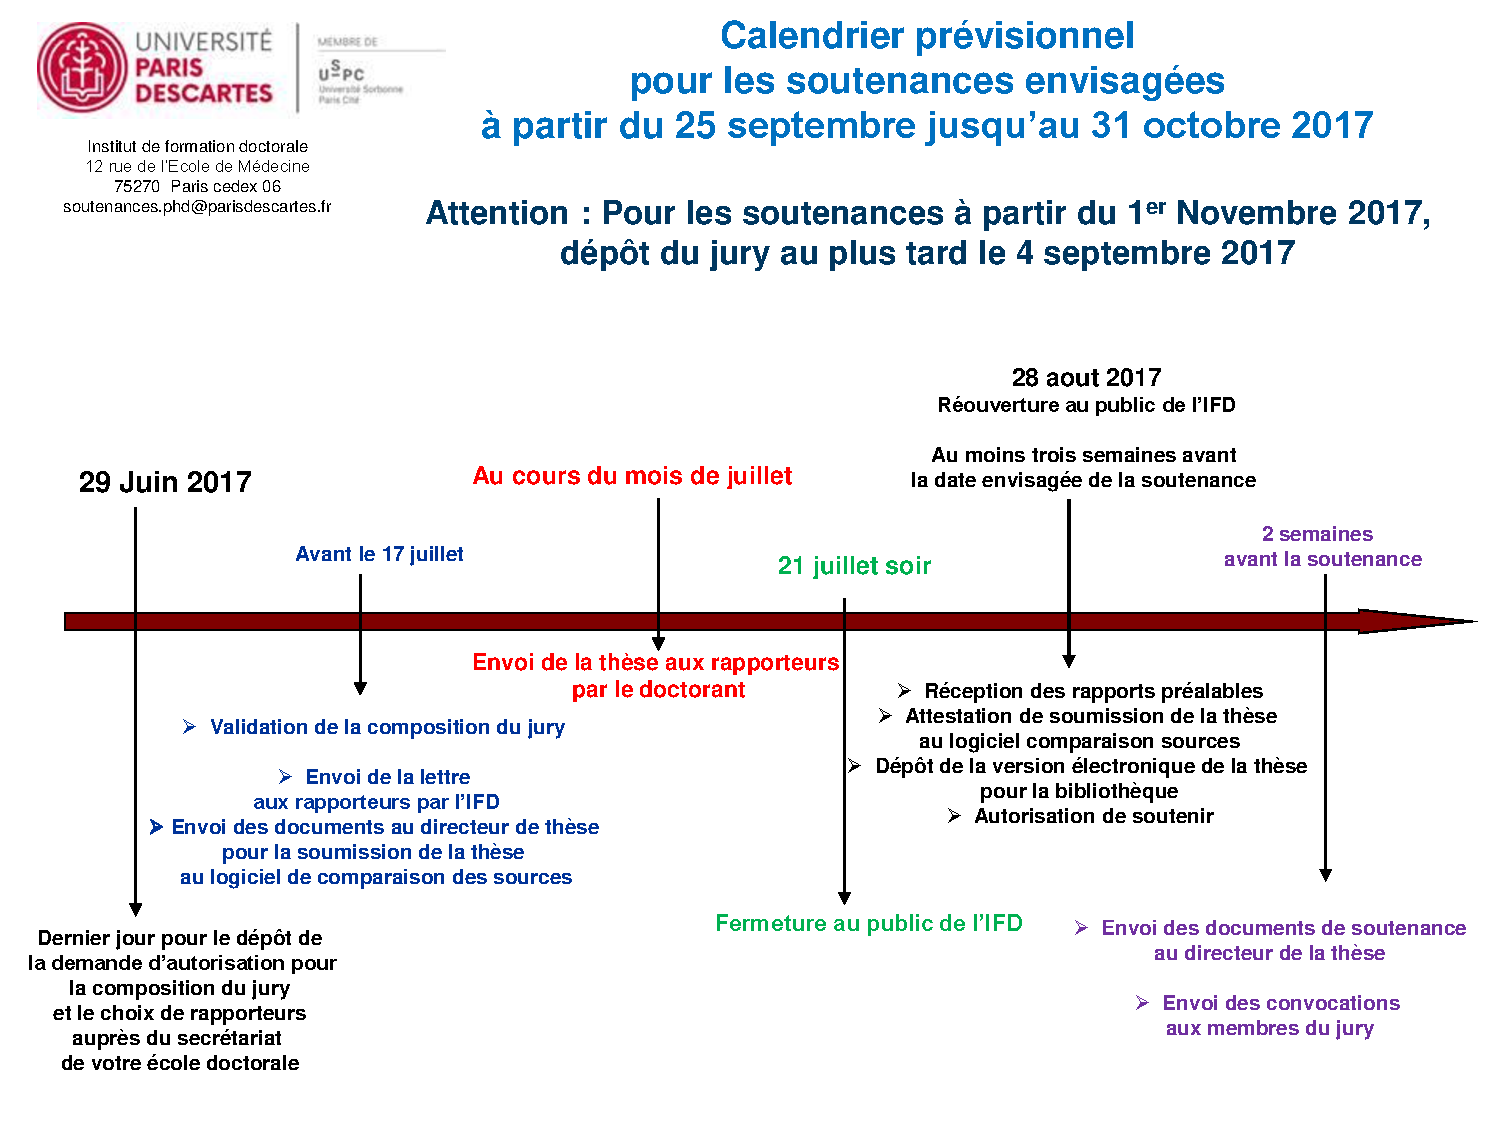
\includegraphics{figures-ext/An-timeline.pdf}
\caption{Timeline provided by University Paris Descartes for 2017}
\end{figure}

\hypertarget{thesis-writing}{%
\section*{Thesis writing}\label{thesis-writing}}
\addcontentsline{toc}{section}{Thesis writing}

This Report is written in
\href{https://github.com/rstudio/bookdown}{\emph{bookdown}}. I have
chosen this form as it can easily compile to \emph{LaTeX}, PDF, MS Word,
ebook and html. Optimally, the final manuscript will be also published
online in a form of an open source
\href{https://www.gitbook.com/about}{gitBook} and an ebook including
interactive figures and maybe even data demos. Another good reason for
using \href{https://github.com/rstudio/bookdown}{\emph{bookdown}} is its
simple syntax of markdown and natural integration of code snippets with
.Rmd. It reduces formatting time and give multiple outputs.

The template of for this thesis manuscript was adapted from \emph{LaTeX}
template provided by University Paris Descartes.

The format \emph{thesis by publication} will be considered for parts of
the thesis.

\newpage

\hypertarget{activity-report-2017}{%
\section*{Activity Report 2017}\label{activity-report-2017}}
\addcontentsline{toc}{section}{Activity Report 2017}

This documents list main achievements of 2017 including conference,
posters and publications list.

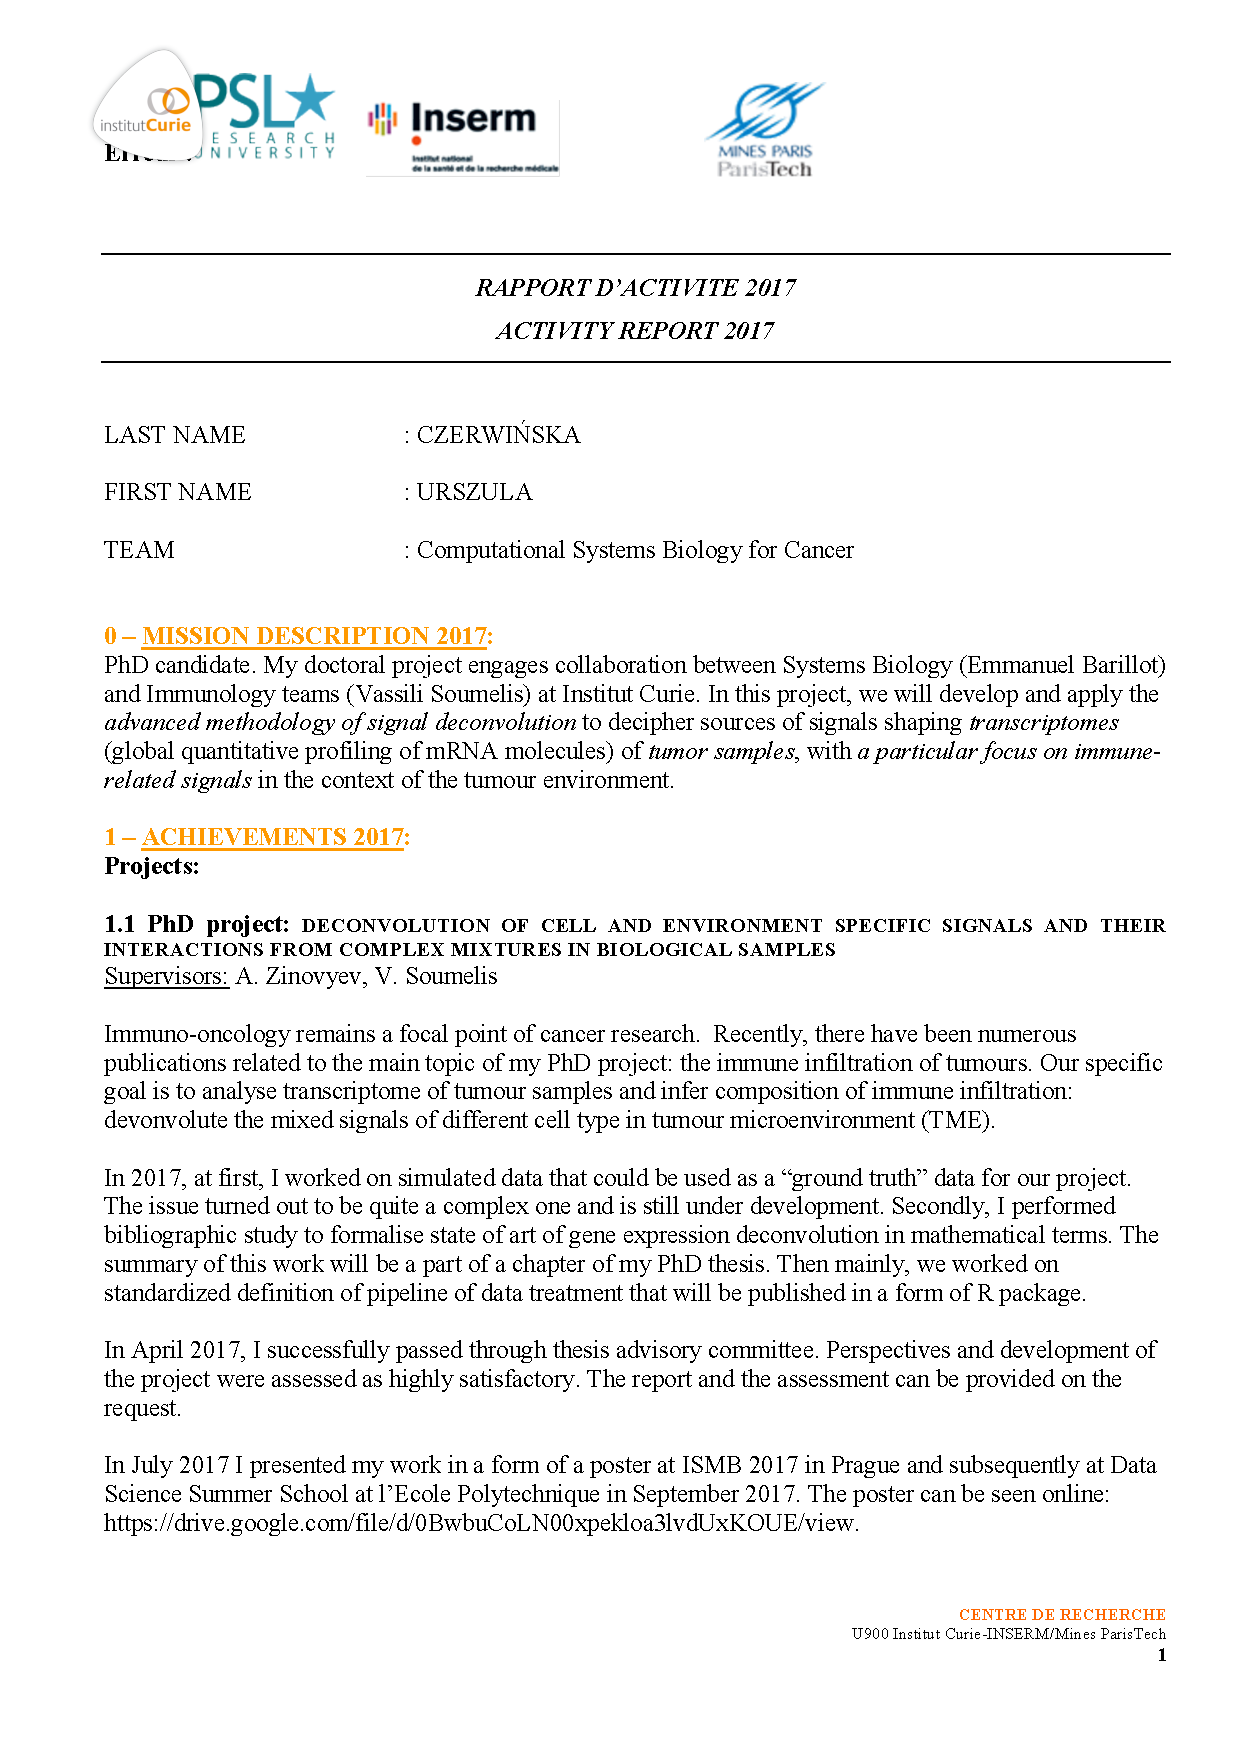
\includepdf[pages={1-}, scale=1]{pdf-ext/An-RA2017.pdf}

\bibliography{book.bib,packages.bib,UCzcite.bib}


\end{document}
